% Reading the Reader paper, merged draft v0.2 (2026-09-06).
% Merged from paper-fable (skeleton, figures, related work), paper-sol (correctness audit),
% and paper-astra (data audit, generated tables, bibliography metadata). See README.md.
% Build: make   (runs the audit-derived asset generation, then latexmk into build/)
% Conventions: British English, first-person plural, one sentence per line, no em dashes.
% Every number in the body comes from generated/results.tex or a generated table unless
% it is a design constant taken from the source code.
%
% Two layouts from one source:
%   make          two-column sigconf reading copy (default; what the authors prefer to read)
%   make review   ETRA review format, confirmed on the ETRA 2026 submission page: single-column
%                 manuscript with line numbers, author-year citations, abstract of at most
%                 150 words, 14 pages for full papers excluding references, anonymous
%                 (ETRA 2027 call: "manuscript,review,anonymous", author-year citations).
% The review build defines \reviewlayout before this file is read (latexmk -usepretex).
\ifdefined\reviewlayout
  \documentclass[manuscript,review,anonymous,screen]{acmart}
  \citestyle{acmauthoryear}
  % Single column: wide and narrow floats are the same environment.
  \newenvironment{widefigure}{\begin{figure}}{\end{figure}}
  \newenvironment{widetable}{\begin{table}}{\end{table}}
  \newcommand{\narrowwidth}{0.5\textwidth}
\else
  \documentclass[sigconf,screen]{acmart}
  % Narrow columns: allow a little extra stretch instead of overfull lines.
  \setlength{\emergencystretch}{2em}
  % Two columns: wide floats span both columns, narrow ones fill one column.
  \newenvironment{widefigure}{\begin{figure*}}{\end{figure*}}
  \newenvironment{widetable}{\begin{table*}}{\end{table*}}
  \newcommand{\narrowwidth}{0.92\columnwidth}
\fi

\setcopyright{none}
\settopmatter{printacmref=false,printfolios=true}
\renewcommand\footnotetextcopyrightpermission[1]{}
\acmConference[ETRA '27]{2027 Symposium on Eye Tracking Research and Applications}{June 7--10, 2027}{Pamplona, Spain}
\acmYear{2027}

\usepackage{booktabs}

% Black hyperlinks (citation numbers, cross-references, URLs, emails): the class
% colours them purple and blue for the screen build. Must run after the class's
% own \hypersetup, which it issues at the end of the preamble.
\AtBeginDocument{\hypersetup{allcolors=black}}

% Audited numbers and generated tables (regenerate with: make assets).
% Generated by analysis/build_paper_assets.py; do not edit by hand.
\newcommand{\participantsN}{4}
\newcommand{\sessionsN}{8}
\newcommand{\gazeTotal}{175,860}
\newcommand{\gazeMeanHz}{89.89}
\newcommand{\gazeSdHz}{0.21}
\newcommand{\gazeMinHz}{89.41}
\newcommand{\gazeMaxHz}{90.06}
\newcommand{\gazeMeanValid}{95.6}
\newcommand{\gazeMinValid}{92.5}
\newcommand{\gazeMaxValid}{98.0}
\newcommand{\calAccMin}{0.30}
\newcommand{\calAccMax}{0.69}
\newcommand{\calPrecMin}{0.08}
\newcommand{\calPrecMax}{0.33}
\newcommand{\fixationTotal}{9,311}
\newcommand{\saccadeTotal}{3,225}
\newcommand{\duplicateFixations}{280}
\newcommand{\duplicateSaccades}{652}
\newcommand{\duplicateFixationPct}{3.0}
\newcommand{\duplicateSaccadePct}{20.2}
\newcommand{\interventionsWith}{19}
\newcommand{\interventionsWithout}{26}
\newcommand{\interventionsTotal}{45}
\newcommand{\orderWithFirst}{1}
\newcommand{\orderWithoutFirst}{3}
\newcommand{\rrtWithMedian}{482}
\newcommand{\rrtWithMean}{670}
\newcommand{\rrtWithObserved}{19}
\newcommand{\rrtWithoutMedian}{650}
\newcommand{\rrtWithoutMean}{923}
\newcommand{\rrtWithoutObserved}{25}
\newcommand{\regWithPre}{29.3}
\newcommand{\regWithPost}{22.8}
\newcommand{\regWithoutPre}{32.0}
\newcommand{\regWithoutPost}{33.0}
\newcommand{\regWithPreDedup}{30.9}
\newcommand{\regWithPostDedup}{23.0}
\newcommand{\regWithoutPreDedup}{32.7}
\newcommand{\regWithoutPostDedup}{33.0}
\newcommand{\identityDuplicateFixations}{350}
\newcommand{\identityDuplicateSaccades}{755}
\newcommand{\identityDuplicateFixationPct}{3.8}
\newcommand{\identityDuplicateSaccadePct}{23.4}
\newcommand{\nearDuplicateFixations}{70}
\newcommand{\nearDuplicateSaccades}{103}
\newcommand{\regWithPreIdDedup}{27.2}
\newcommand{\regWithPostIdDedup}{22.9}
\newcommand{\regWithoutPreIdDedup}{31.5}
\newcommand{\regWithoutPostIdDedup}{31.9}
\newcommand{\rrtWithMedianIdDedup}{482}
\newcommand{\rrtWithoutMedianIdDedup}{650}
\newcommand{\rttParticipantN}{387}
\newcommand{\rttParticipantMedian}{1}
\newcommand{\rttParticipantPninefive}{3}
\newcommand{\rttParticipantMax}{41}
\newcommand{\rttResearcherN}{393}
\newcommand{\rttResearcherMedian}{1}
\newcommand{\rttResearcherPninefive}{8.4}
\newcommand{\rttResearcherMax}{28}
\newcommand{\rttCohortN}{780}
\newcommand{\rttCohortOverBudget}{0}
\newcommand{\advDurationS}{91.2}
\newcommand{\advGazeSamples}{8,004}
\newcommand{\advFreshnessN}{14,015}
\newcommand{\advFreshnessMedian}{6}
\newcommand{\advFreshnessPninefive}{11}
\newcommand{\advFreshnessMax}{46}
\newcommand{\advProviderN}{8}
\newcommand{\advProviderMedian}{4.5}
\newcommand{\advProviderMax}{7}
\newcommand{\advParticipantN}{17}
\newcommand{\advParticipantMax}{315}
\newcommand{\advParticipantOverBudget}{1}
\newcommand{\advProposalRecords}{16}
\newcommand{\advUniqueProposals}{8}
\newcommand{\advProposalsApproved}{2}
\newcommand{\advProposalsSuperseded}{6}
\newcommand{\cpPreserved}{3}
\newcommand{\cpDegraded}{16}
\newcommand{\cpDegradedResidualMedian}{389}
\newcommand{\cpDegradedInducedMedian}{38.7}
\newcommand{\sweepTrials}{66}
\newcommand{\sweepPairsOriginal}{62}
\newcommand{\sweepPairsRevised}{63}
\newcommand{\sweepOverOriginal}{45}
\newcommand{\sweepOverRevised}{4}
\newcommand{\sweepOffMedianOriginal}{32.4}
\newcommand{\sweepOffMedianRevised}{34.3}
\newcommand{\sweepOnMedianOriginal}{104.4}
\newcommand{\sweepOnMedianRevised}{32.4}
\newcommand{\sweepAnchorDiff}{21}
\newcommand{\sweepOffDiff}{26}


% Condition labels used by the generated tables.
\newcommand{\on}{\textsc{on}}
\newcommand{\off}{\textsc{off}}

% Visible draft marker for items only the authors can settle.
\newcommand{\todopaper}[1]{\textcolor{red}{\textbf{[TODO: #1]}}}

\begin{document}

\title[Adapt Without Losing the Reader]{Adapt Without Losing the Reader: A Modular Two-Screen Platform for Gaze-Contingent Reading Experiments}
% Alternative titles (see outline.md):
% - A Researcher-Operated Platform for Real-Time, Context-Preserving Typographic Interventions
% - From Prototype to Instrument: Modular Infrastructure for Gaze-Adaptive Reading Research

% Affiliation format as requested by Ashkan Tashk (2026-10-07). The co-authors are entered in
% the submission system only; for the camera-ready add them here in the agreed order:
% Sachin Baral, Satish Gurung, Ashkan Tashk, Chaudhary Muhammad Aqdus Ilyas, Per Baekgaard.
\author{Sachin Baral}
\affiliation{%
  \department{Department of Applied Mathematics and Computer Science (DTU Compute)}
  \institution{Technical University of Denmark (DTU)}
  \city{Kgs. Lyngby}
  \country{Denmark}}
\email{s243871@dtu.dk}

\author{Satish Gurung}
\affiliation{%
  \department{Department of Applied Mathematics and Computer Science (DTU Compute)}
  \institution{Technical University of Denmark (DTU)}
  \city{Kgs. Lyngby}
  \country{Denmark}}
\email{s243872@dtu.dk}

\renewcommand{\shortauthors}{Baral and Gurung}

\begin{abstract}
Gaze-driven text adaptation has been demonstrated repeatedly, but existing prototypes couple sensing, decision logic, and presentation, so comparing interventions remains expensive.
We present a researcher-operated, two-screen platform whose sensing, eye-movement analysis, decision, and intervention stages are replaceable modules behind stable contracts.
A participant reads reflowable text that adapts to their gaze while a researcher mirrors the reading live and applies or approves typographic changes; every sample, proposal, intervention, and restoration outcome enters one replayable record.
Across eight Tobii sessions, the platform sustained a rated 90\,Hz, kept gaze validity above 92\%, kept all 780 client round trips below 100\,ms, and ran a collaborator's reading-difficulty pipeline as its live analysis module.
Because the platform records every intervention's positional cost, it showed that our original context-preserving restore moved readers about three times farther than the reflow it compensated; we describe the revision and its geometric evidence.
\end{abstract}

% TODO(authors): regenerate the CCS concepts with the ACM CCS tool (dl.acm.org/ccs) before submission.
\begin{CCSXML}
<ccs2012>
<concept>
<concept_id>10003120.10003121.10003129</concept_id>
<concept_desc>Human-centered computing~Interactive systems and tools</concept_desc>
<concept_significance>500</concept_significance>
</concept>
<concept>
<concept_id>10003120.10003121.10011748</concept_id>
<concept_desc>Human-centered computing~Empirical studies in HCI</concept_desc>
<concept_significance>300</concept_significance>
</concept>
<concept>
<concept_id>10003120.10011738.10011775</concept_id>
<concept_desc>Human-centered computing~Accessibility systems and tools</concept_desc>
<concept_significance>300</concept_significance>
</concept>
</ccs2012>
\end{CCSXML}

\ccsdesc[500]{Human-centered computing~Interactive systems and tools}
\ccsdesc[300]{Human-centered computing~Empirical studies in HCI}
\ccsdesc[300]{Human-centered computing~Accessibility systems and tools}

\keywords{eye tracking, adaptive reading, gaze-contingent interfaces, typographic interventions, context preservation, research platforms}

\begin{teaserfigure}
  \centering
  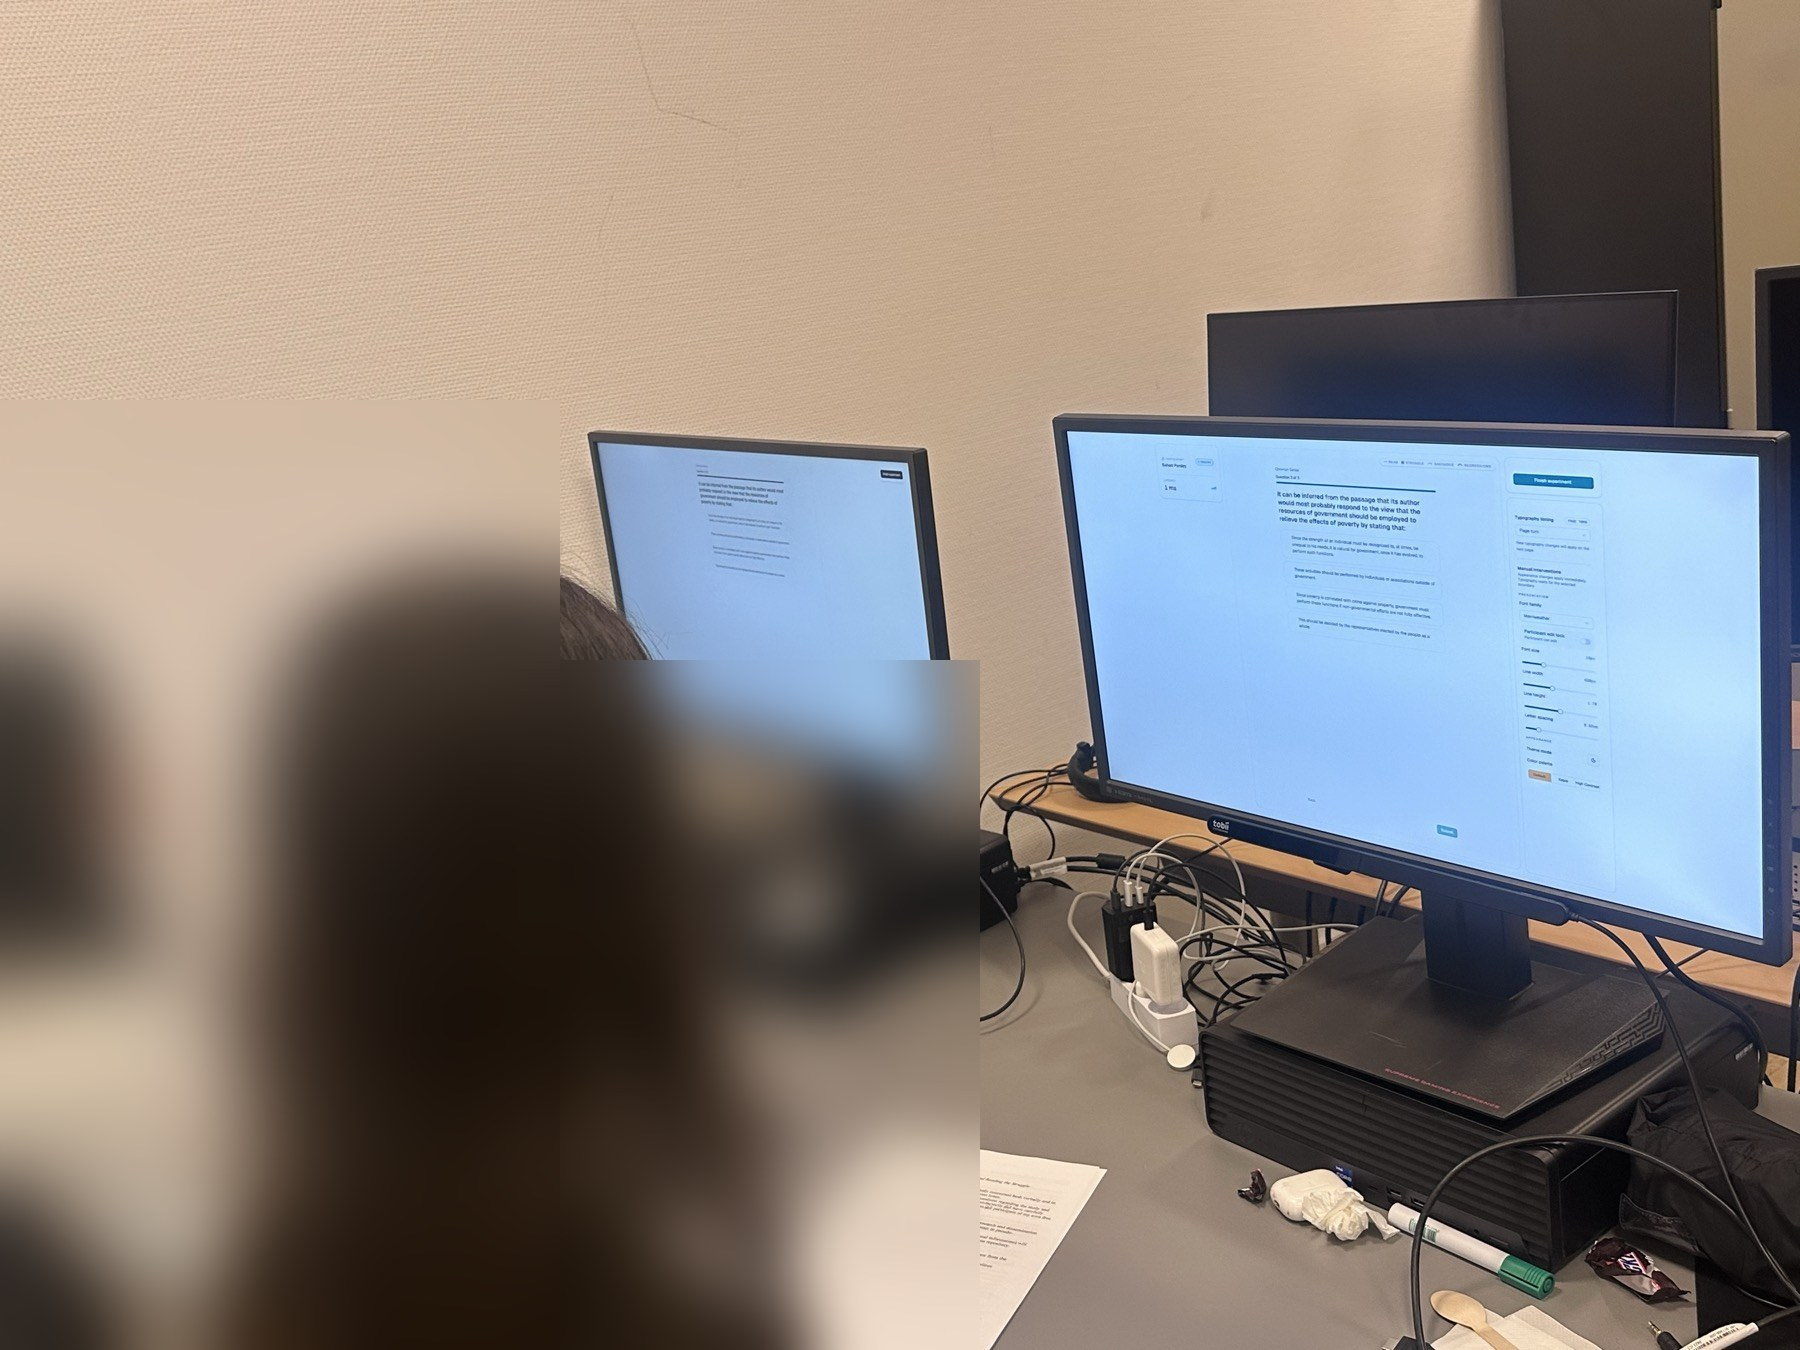
\includegraphics[width=0.52\textwidth]{figures/experiment-setup.jpg}
  \caption{The two-screen setup during an evaluation session.
  The participant reads the presented text on one display (left), while the researcher monitors the mirrored view and applies interventions from the console on the other (right); the eye tracker is mounted at the foot of the participant's display, and both surfaces are served by one backend on a single host.
  Faces are blurred for anonymity.}
  \Description{A photograph of two desks with monitors. On the left, a participant reads text on a screen with an eye tracker mounted below it. On the right, a researcher operates a console showing the mirrored text and control panels.}
  \label{fig:rig}
\end{teaserfigure}

\maketitle

\section{Introduction}
\label{sec:intro}

Reading underpins participation in education, employment, and daily life, yet for many people it is far from effortless.
The World Health Organization estimates that at least 2.2 billion people live with a vision impairment \cite{who2026vision}, age-related macular degeneration alone is projected to affect 288 million people by 2040 \cite{apte2021amd}, and reading difficulties such as dyslexia add to the population for whom text demands more than the visual or cognitive system can comfortably supply.
Digital text offers a response that print cannot: its presentation can change while it is being read.
Font size, spacing, line length, and contrast are all adjustable on screen, controlled readability studies show that such parameters measurably affect reading \cite{rello2016makeitbig, beymer2008eyetracking, beier2021letterspacing}, and an eye tracker supplies the moment-to-moment signal needed to apply an adjustment exactly when a reader needs it.
A system that couples the two can deliver individualised typographic micro-interventions \cite{persson2025microintervention} without the reader ever issuing a command.

The promise carries a structural risk.
A typographic change that helps in principle also reflows the document, so the line a participant was reading moves, and an ill-timed change costs the reader their place in the very flow the system is trying to protect.
Prior work confirms both sides of this tension: gaze-driven typographic adaptation is technically achievable, and the design of the intervention, in particular how the transition is presented and whether the reader's context is preserved, measurably shapes recovery and acceptance \cite{pereira2024typography, jensen2025context}.

We argue that the bottleneck in this research area has shifted.
Demonstrating that gaze-driven adaptation works no longer requires another prototype; three generations of adaptive readers in the Reading the Reader programme alone have shown it \cite{refsgaard2024rtr, pereira2024typography, palinec2024reactive}.
What is missing is the instrument for studying it: each of those prototypes wove sensing, decision logic, and the reading interface into one codebase, so each new study extended the previous system by forking it, and none offered a researcher console for operating a controlled session or a session record from which an experiment could be reconstructed.
Consider a researcher who wants to test whether fading a font change gradually into place disrupts a reader less than applying it abruptly.
On a coupled prototype this scientifically simple comparison means editing core application code and maintaining two divergent forks under identical sensing.
An experiment that should be a configuration choice is instead a software project.

This paper presents a platform built to remove that friction, shown in Figure~\ref{fig:rig}.
A participant reads reflowable text on one screen while the text adapts to their gaze; on a second screen, a researcher follows the participant's gaze, fixations, and regressions live over a mirror of the same text, and applies typographic interventions or approves machine-proposed ones during the session.
Behind this workflow, the adaptive loop is decomposed into four independently replaceable modules (sensing, eye-movement analysis, decision strategy, and intervention execution) connected through stable contracts, and every gaze sample, decision, and intervention is written into one schema-versioned session record that can be exported, replayed, and re-analysed.

The contributions are:
\begin{itemize}
  \item \textbf{A modular platform for gaze-contingent reading experiments}, in which sensing, analysis, decision, and intervention are separate modules behind stable contracts, extendable in process by registration and out of process through a documented provider protocol.
  \item \textbf{A two-screen, researcher-in-the-loop workflow}, in which interventions are applied manually, proposed by a decision provider and gated by the researcher (advisory), or applied autonomously, without structural change between modes.
  \item \textbf{A context-preserving intervention mechanism that measures its own cost}: layout changes can be committed at controlled boundaries, a continuously captured anchor restores the reader's position across the reflow, and a graded positional outcome for every intervention is written into the session record.
  \item \textbf{A technical evaluation on real eye-tracking hardware} covering capture and transport, external-provider integration (including a collaborator's reading-difficulty pipeline that analysed the evaluation sessions live), and context preservation, whose self-measurement exposed a defect in our original restore strategy that over-repositioned the reader on small reflows; we describe the revision and its geometric evidence.
\end{itemize}

We report the evaluation as an evaluation of the instrument: with four participants the behavioural observations are descriptive, and the paper makes no claim that any intervention improves reading.
The platform, its documentation, and the audit script that regenerates every quantity in this paper from the exported records are openly available.

\section{Related Work}
\label{sec:related}

\subsection{Gaze-Contingent and Adaptive Reading}

Using the reader's gaze to change the reading experience in real time has a long line of demonstrations.
The eyeBook coupled an eye tracker to a digital book to trigger in-situ effects as the reader progressed \cite{biedert2010eyebook}.
More recently, \citet{medan2024newline} presented text as a single line that scrolls with the reader's webcam-estimated gaze and emphasises the fixated word; a pilot with 13 participants found no significant change in comprehension or speed but a clear preference for the interface.
\citet{rummens2026highlighting} coloured the word under fixation in real time for seventy second graders reading aloud and reported faster reading with shorter fixations, fewer regressions, and less re-reading, without loss of pronunciation accuracy or comprehension, although the children preferred the static text.
That split between performance and preference is a useful reporting model for adaptive reading.
Gaze during reading is also used as a measurement instrument in its own right, for example to compare how readers process AI-generated and human-authored text \cite{ilyas2025mind}.

Within the Reading the Reader programme, three master's projects built successive adaptive readers: a flexible reading and gaze-collection application \cite{refsgaard2024rtr}, an adaptive e-reader used to compare four intervention presentation forms, which were found to differ substantially in disruption and acceptance \cite{pereira2024typography}, and a reactive frontend designed to consume machine-learning output \cite{palinec2024reactive}.
\citet{jensen2025context} then showed that context preservation is where intervention design bites: in a 22-participant within-subjects study of four intervention designs they introduced reading-resume time as a recovery measure and reported that a gradual transition combined with context highlighting resumed fastest, reducing the time lost to an intervention from 14.9\,s to 4.0\,s, and was the most preferred design.
Each of these systems, however, was built for its own study.
Sensing, decision logic, and presentation were coupled in one application, so the next study copied and modified the previous system rather than reconfiguring a shared one.
Our platform is the infrastructural complement to this line of work: it is built so that exactly such comparisons of intervention designs can be run, varied, and reconstructed without touching core code.

\subsection{Real-Time Gaze Processing for Reading}

Reducing a raw gaze stream to oculomotor events is the classical first step, with identification algorithms catalogued by velocity, dispersion, and area-of-interest families \cite{salvucci2000identifying} and reading behaviour extensively characterised \cite{rayner1998eyemovements}.
Real-time use sharpens the problem: noisy vertical gaze must be assigned to the correct line while the reader is still reading.
\citet{kaltenberger2026line} address this with CONF-LA, a confidence-scored online fixation-to-line assignment that defers uncertain assignments.
Our contribution on this front is architectural rather than algorithmic.
The platform's built-in analysis is a dwell-based, token-level area-of-interest method whose spatial half hit-tests gaze against the words' live on-screen boxes (Section~\ref{sec:platform-mapping}), so a typographic reflow cannot invalidate the mapping; and the whole analysis stage is a replaceable, logged strategy, so a stronger detector or a confidence-aware line-assignment method can be attached as a provider without modifying the platform.
We do not claim token-level assignment accuracy for the built-in heuristic, which has not been validated against ground truth.

\subsection{Experiment Tooling}

A researcher building a reading study today would more likely reach for general-purpose experiment software than for a research prototype.
Tobii Pro Lab \cite{tobii2025prolab}, PsychoPy \cite{peirce2019psychopy}, OpenSesame \cite{mathot2012opensesame}, and Psychtoolbox \cite{brainard1997psychtoolbox} are mature platforms for experiment design, stimulus delivery, and gaze capture, and PsychoPy's ioHub already offers a common interface across tracker vendors together with a simulated mouse-driven gaze source \cite{psychopy2026iohub}, so hardware abstraction and simulated gaze are not in themselves new.
Two recent ETRA contributions show the same open-source tooling trend at both ends of the sensing chain.
\citet{salari2026pyelink} provide PyeLink and SyeLink, Python tools that expose low-level control of EyeLink trackers to Pygame, PsychoPy, and Pyglet experiments, including recording during calibration and raw pupil and corneal-reflection data, and that parse the resulting files into structured data; \citet{salari2026pyetsimul} provide PyEtSimul, a simulator of video-based eye trackers that generates synthetic eye features from a geometric model so that gaze-estimation algorithms can be benchmarked reproducibly without hardware or participants.
Both sit below the reading loop: they broaden what a sensing stage can be, and they are the kind of component our sensing port is designed to admit (Section~\ref{sec:platform-mapping}).
What these tools leave to study-specific programming is the reading-specific loop: mapping gaze onto reflowable text, proposing and gating typographic changes, committing them without losing the reader, and measuring what the change cost.
Table~\ref{tab:capability} summarises the authors' assessment of the three most established tools against the capabilities a gaze-driven reading experiment requires; none closes the loop from live gaze to a typographic change in the text being read, and none exposes a pluggable decision boundary.
Our platform occupies that region as a focused instrument for one family of experiments; it complements rather than replaces the general-purpose tools.

% TODO(authors): re-verify the Partial/No ratings against current primary documentation before submission.
\begin{widetable}
\centering
\small
\caption{Capability comparison of established experiment software with our platform, across the capabilities a gaze-driven reading experiment requires.
Entries reflect the authors' assessment of documented capabilities \cite{tobii2025prolab, peirce2019psychopy, brainard1997psychtoolbox}.}
\label{tab:capability}
\begin{tabular}{@{}lcccc@{}}
\toprule
Capability & Tobii Pro Lab & PsychoPy & Psychtoolbox & This platform \\
\midrule
Design experiments & Yes & Yes & Yes & Yes \\
Record gaze data & Yes & Partial & Partial & Yes \\
Analyse recorded data & Yes & Partial & No & Yes \\
Real-time gaze-driven text intervention & No & Partial & Partial & Yes \\
Pluggable decision modules & No & No & No & Yes \\
\bottomrule
\end{tabular}
\end{widetable}

\section{The Platform}
\label{sec:platform}

\subsection{Overview: One Loop, Four Modules, Two Screens}
\label{sec:platform-overview}

The platform decomposes the adaptive reading loop into four concerns chosen along the axis of replaceability: \emph{sensing} produces a continuous stream of gaze samples; \emph{analysis} projects that stream into oculomotor events (fixations, saccades, regressions); \emph{decision} consumes the analysed state and returns at most a proposal to intervene; and \emph{intervention} validates a proposal and commits a change to the text.
Each concern sits behind a stable contract with a uniform shape: a module is identified by a stable provider identity and exposes a single operation that receives an immutable snapshot of the relevant session state and returns an optional result.
Because a module is handed a copy of what it needs rather than a reference to live state, it can neither reach into nor mutate the core; and because the runtime resolves modules from a per-concern registry by identifier, never naming a concrete implementation, adding an in-process module is one registration and no existing code changes.
The .NET backend owns all authoritative session state; within its application assembly the four boundaries are contracts and registries, not separately deployed units, and the build enforces the dependency rule (Section~\ref{sec:eval-modularity}).
The platform was implemented by the authors with generative AI coding assistance, as described in the disclosure at the end of the paper.

Two browser surfaces of a single web frontend face the two people in the room (Figure~\ref{fig:screens}).
The participant surface renders the reading material as reflowable, tokenised text.
The researcher console mirrors the same text and overlays the participant's live gaze, a fixation heat map, and recent saccades, so the researcher sees not merely where the participant looks but how they read.
The surfaces never communicate with each other; both render the same backend-owned snapshot, so they cannot disagree.
Discrete commands (configure a session, change an intervention policy, start, stop) travel over a request-and-response channel, while the high-frequency gaze stream travels over a separate real-time channel (a single WebSocket per client), a split that keeps the per-sample path away from the lock that serialises session lifecycle commands.
One cycle of the loop runs across these parts: a gaze sample is mirrored to both surfaces; the participant surface, which alone knows the rendered layout, maps it to a token and returns an enriched observation; analysis projects observations into oculomotor events; a decision (built-in, external, or the researcher acting manually) yields at most one proposal, which in advisory mode waits for approval; and the intervention commits at its configured boundary, after which the adapted text returns to both surfaces while persistence checkpoints are written throughout.

\begin{widefigure}
  \centering
  % Equal heights put the two screenshots at the same scale: the reading column is the same
  % fraction of each screenshot's height, so the mirrored text is as large as the participant's.
  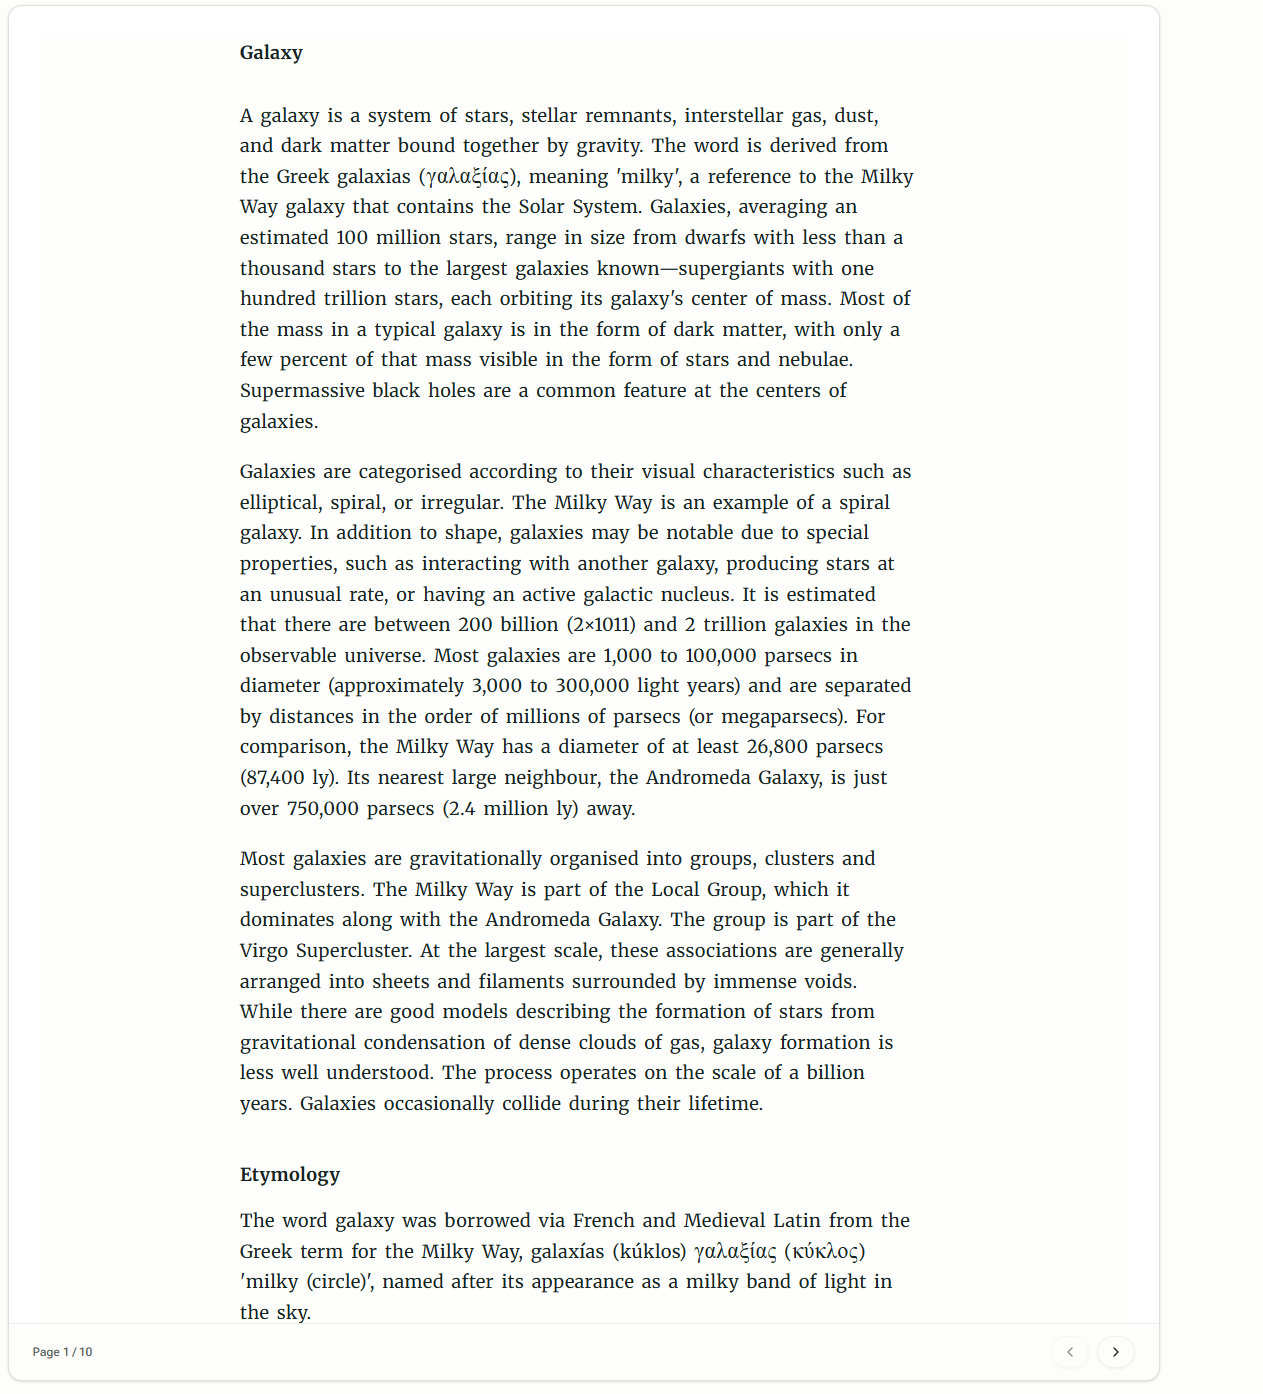
\includegraphics[height=0.44\textwidth]{figures/ReadingView.png}\hspace{0.02\textwidth}
  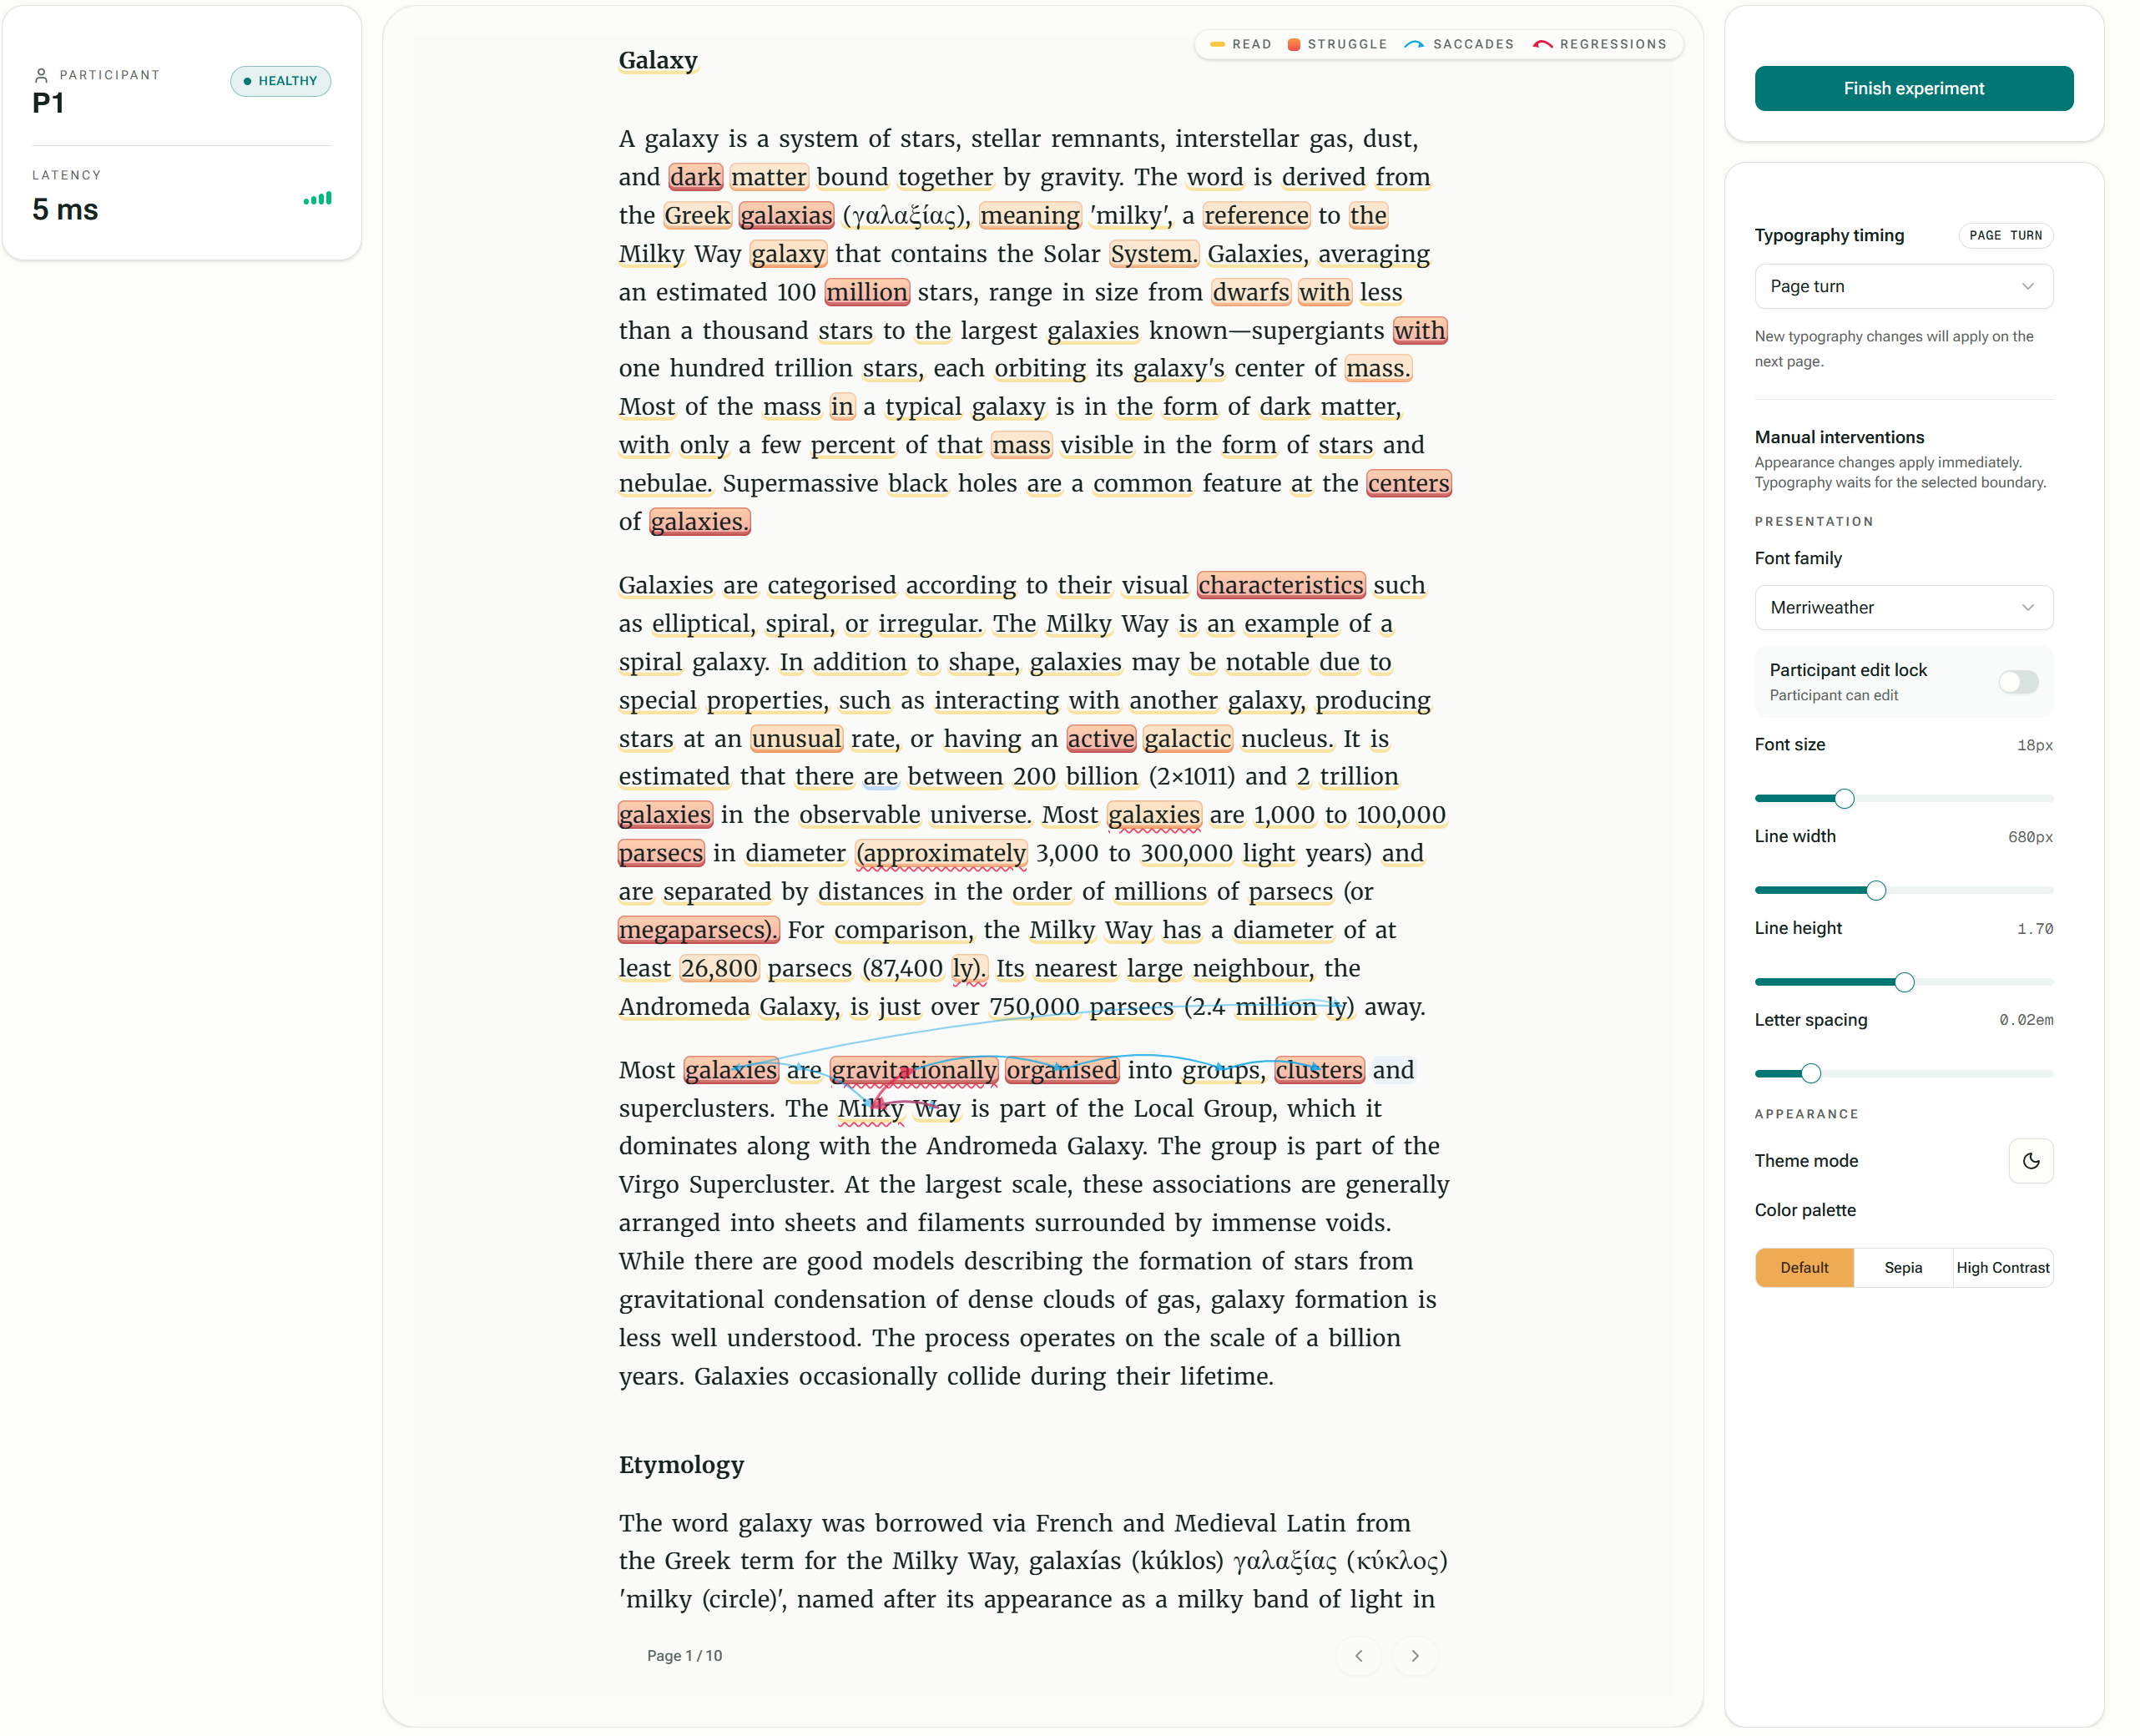
\includegraphics[height=0.44\textwidth]{figures/ResearcherLiveView.png}
  \caption{The two operated surfaces at the same scale: the participant reader (left) and the researcher console mirroring the same text with live gaze, fixation, and saccade overlays and the intervention controls (right).}
  \Description{Two application screenshots side by side. The left shows a clean reading view with a paragraph of text. The right shows the same text overlaid with gaze markers and, beside it, control panels for interventions and session state.}
  \label{fig:screens}
\end{widefigure}

\subsection{Sensing and Gaze-to-Word Mapping}
\label{sec:platform-mapping}

Sensing is a port with interchangeable sources.
The primary adapter subscribes to a Tobii eye tracker's native callback and republishes each sample (per-eye position on the display area normalised to the unit square, pupil data, validity flags, device timestamp) into the domain; a simulated source emits samples of exactly the same shape from the mouse cursor, so the full loop runs with or without hardware and the downstream stages cannot tell which source produced a sample.
The port is deliberately narrow so that other sources fit behind it: an adapter over a low-level tracker interface such as PyeLink \cite{salari2026pyelink} would add EyeLink hardware, and a synthetic stream of the kind PyEtSimul \cite{salari2026pyetsimul} generates would let the loop be exercised under controlled, reproducible gaze without an eye tracker in the room; neither adapter has been implemented, and we claim only that the seam admits them.
On the backend the per-sample path avoids the lifecycle lock: each arriving sample is sanitised, published with a volatile write as the latest value, counted atomically, and broadcast, while appending it to the session history takes a separate, short history lock.
The heavier modular pipeline of analysis, decision, and intervention runs at the cadence of analysed-state changes rather than once per raw sample, which keeps the indirection introduced for modularity off the per-sample path, and the participant surface coalesces snapshot bursts to one render per animation frame.

The spatial half of the pipeline runs in the reader, the only place the rendered layout exists.
Every word is a tokenised span whose on-screen box is measured from the live DOM and re-measured whenever the layout changes, prompted by mutation, resize, and scroll observers.
An incoming gaze point is smoothed adaptively, mapped into the reading area, and hit-tested in two stages: first the line, scored by vertical distance with a fixed hysteresis bonus for the line currently being read, so that vertical jitter of the order of the line spacing does not flicker attribution between neighbours; then the nearest word on that line.
The mapping has two properties that matter for an adaptive reader.
It is resolution-independent, because the tracker reports gaze as a fraction of the display and the words are measured live rather than assumed.
And it is reflow-proof by construction: a typographic intervention that moves every word to a new position cannot invalidate the mapping, because the next sample is hit-tested against the boxes as they now are, which is precisely the failure mode a coordinate-based scheme would suffer.
The heuristic's thresholds are hand-tuned and its token-level accuracy has not been validated against ground truth; it is a replaceable component.
The result of the stage is a token-level reading observation (token, line, and block identity) published back to the backend.

\subsection{Eye-Movement Analysis as a Replaceable Strategy}
\label{sec:platform-analysis}

The temporal half of the pipeline is an explicit analysis strategy behind its own contract.
The built-in strategy realises the area-of-interest branch of the classical taxonomy \cite{salvucci2000identifying}: since each observation is already bound to a word, the word itself is the area of interest, a fixation is confirmed from accumulated dwell against thresholds that are raised across a line change because cross-line movement is noisier, and per-word statistics separate read words from skimmed ones by dwell.
Saccades are classified from token and line deltas, and a backward or line-change-backward saccade is counted as a regression, the standard oculomotor sign of reading disruption \cite{rayner1998eyemovements}.
The strategy is a pure function of the observation and the prior state, so replaying the same observations yields the same events, and it is resolved from a registry, so an external analysis provider can replace it at runtime (Section~\ref{sec:platform-decision}).

\subsection{The Decision Boundary and Execution Modes}
\label{sec:platform-decision}

Decisions about when and how to adapt the text can come from three sources: the researcher acting manually from the console, a built-in rule-based strategy, or an external provider.
Two execution modes cover the supervision spectrum without structural change: in \emph{advisory} mode every machine proposal is surfaced on the console and applied only when the researcher approves it, and in \emph{autonomous} mode a permitted proposal is applied directly.
Every proposal passes through an explicit lifecycle with exactly one terminal outcome (approved, rejected, applied, or superseded when a newer proposal or a mode change overtakes it), so the text never adapts on a decision that no longer holds, and every outcome is logged.
In all modes the intervention runtime validates the requested change independently: it normalises the parameter against the current presentation, bounds the step, and applies cooldown rules to automated proposals, so a faulty provider cannot bypass the guardrails.

External providers connect out of process over a documented WebSocket protocol: a handshake in which the provider declares its identity, modules, and capabilities and receives an accept-or-reject reply, followed by heartbeats and tunnelled traffic.
What crosses the boundary is a fixed vocabulary: outward, an immutable session snapshot and the stream of analysed signals (reading focus, attention summary, oculomotor events); inward, a proposal pairing an observed signal and a short human-readable rationale with the identity of an intervention module and the parameters to apply.
The seam commits the platform to signals in and a proposal out, but not to any particular way of arriving at the proposal, which is what makes an AI-driven provider a configuration rather than a rewrite.
An external decision is applied through exactly the same validation and logging path as a built-in one.
When a provider disconnects, the platform marks it detached, records the transition as a lifecycle event, and the session continues; the current runtime does not switch the affected concern to its built-in strategy on its own, and although the handshake advertises a heartbeat timeout, heartbeats are recorded rather than enforced.
The same provider framework serves the analysis seam in the same way, one mechanism for two concerns.

\subsection{Context-Preserving Interventions}
\label{sec:platform-context}

Typographic interventions are the platform's actuator: built-in modules cover font family, font size, line width, line height, letter spacing, theme, and palette.
Appearance-only changes commit immediately.
A layout-changing intervention can be committed immediately or held until a chosen boundary (the end of the sentence or paragraph being read, or the page turn), so that a reflow can land at a natural break rather than mid-line.

Around the commit, the reader runs a capture-and-restore mechanism.
An anchor is captured continuously (every 120\,ms and on content changes), preferring the word the participant is currently reading, degrading to a visible fallback word or its enclosing block, and recording the element's identity together with its viewport offset; anchors older than 15\,s are rejected as stale.
When a layout change commits, the reader re-locates the anchor in the reflowed document (degrading sentence to token to block) and scrolls it back to the viewport offset it held before the change.
The residual error between target and achieved offset is then measured, graded (preserved, degraded, or failed, with tolerances of 72\,px for a full reflow and 48\,px to 120\,px otherwise), and written into the session record next to the intervention that caused it, together with the displacement the reflow itself induced.
Optionally, the restored sentence is briefly highlighted and fades over about three seconds, drawing the eye back to the resume point, which corresponds to the highlighting component that prior work found effective for recovery \cite{jensen2025context}.
Because the sentence is re-located before the token, a small sentence-anchor residual does not by itself guarantee that the word being read stayed still; the evaluation therefore measures word displacement directly (Section~\ref{sec:eval-context}).

Section~\ref{sec:eval-context} shows how these recorded outcomes exposed a defect in our original restore strategy.
Because every intervention's graded outcome and residual are in the record, a later analysis can ask not only whether an intervention helped a reader but what it cost them in lost position.

\subsection{Researcher Console, Session Record, and Replay}
\label{sec:platform-record}

A session is operated end to end from the researcher console.
Setup is a gated stepper: a session cannot start until a participant is saved, a licensed eye tracker is selected, a calibration (9-, 13-, or 16-point presets with a five-target accuracy and precision validation) has passed, and reading material is chosen, with the gates re-checked by the backend at the moment of start.
During the run, the console shows the mirror with live analysis overlays, the gaze-validity rate, and the measured client round-trip time, and carries the intervention and typography controls together with the approval queue in advisory mode.

Everything that happens flows into one authoritative, schema-versioned session record owned by the backend: run parameters and presentation baseline, calibration metrics, screen geometry, the raw gaze stream, derived oculomotor events, decision proposals and their outcomes, interventions and their context-preservation outcomes, and quiz responses, each entry stamped with a monotonic sequence number and timestamp.
The record is the same structure a background worker checkpoints throughout the session, so durability and export are one artifact and an interrupted session is recoverable from its latest checkpoint.
A completed record exports to JSON and CSV, re-imports through a version-gated schema check, and replays in the reading interface with scrubbing, variable speed, and jump-to-event navigation.
Replay reconstructs the recorded events at any instant; reproducing a study in the scientific sense additionally requires the code, provider, and configuration versions, which the export records only in part (its manifest names the producing application and tracker SDK versions, and its condition fields come from the final session snapshot).
A separate telemetry record (client round-trip times, achieved sampling rate, validity, and decision-path timings) against an explicit 100\,ms budget is the instrumentation behind Section~\ref{sec:eval-perf}.

\section{Evaluation}
\label{sec:eval}

The evaluation asks three questions that mirror the platform's claims: whether the four concerns are genuinely replaceable without touching the core (Section~\ref{sec:eval-modularity}), whether a real eye-tracking stream drives the loop with measurable quality and transport delay (Section~\ref{sec:eval-perf}), and whether interventions can adapt the text while preserving the reader's context (Section~\ref{sec:eval-context}).
The scope is architecture and runtime feasibility, not human efficacy: with \participantsN{} participants, the behavioural numbers below are descriptive, and we draw no statistical inference from them.
Every quantity, table, and figure in this section is derived from the exported session and telemetry records by a dependency-free audit script committed with the paper; the script records the SHA-256 hash of each of its 20 input files and reproduces the summaries of the thesis analysis to numerical precision.

\subsection{Setup}
\label{sec:eval-setup}

We recorded \sessionsN{} reading sessions on real hardware: \participantsN{} participants each read under two conditions, with the context-preserving restore enabled (\on{}) and disabled (\off{}), as summarised in Table~\ref{tab:sessions}.
Two expository Markdown articles were used (\emph{Metal Detectors} and \emph{Nuclear Science}); each participant read a different article in each condition, and each article appears twice per condition.
Condition order was not counterbalanced: \orderWithFirst{} participant read the \on{} session first and \orderWithoutFirst{} read the \off{} session first.
Sessions ran on a Tobii \texttt{IS4\_Large\_Peripheral} tracker under a 2560$\times$1440 display, each gated by a passing nine-point calibration validation (average accuracy \calAccMin{} to \calAccMax{} degrees, precision \calPrecMin{} to \calPrecMax{} degrees).
The deployment was the intended single-operator setting: backend and both surfaces on one host, traffic over the local loopback.
All \interventionsTotal{} recorded interventions were applied manually from the researcher console with the immediate commit boundary, so the sessions exercise the manual path and the restore mechanism but not boundary scheduling or automated decisions; one export carries a rule-based advisory configuration in its final metadata although all of its interventions are manual, because condition metadata is taken from the final session snapshot.
Eye-movement analysis in all \sessionsN{} sessions was served live by the collaborator's external provider of Section~\ref{sec:eval-modularity}.
One additional session under an advisory decision strategy exercised the decision-path instrumentation and is reported separately in Section~\ref{sec:eval-perf}.
Every session was operated end to end from the gated researcher console, and every quantity in this section was recomputed from the exported session and telemetry records alone by the audit script, with telemetry joined to exports by session identifier and every context-preservation outcome linked to its intervention.

\begin{widetable}
\centering
\small
\caption{The \sessionsN{} recorded sessions.
Text M is \emph{Metal Detectors} and N is \emph{Nuclear Science}; \on{} bundles positional restoration with the highlight cue.
Duration covers the exported session including activities beyond reading; rate is computed from device timestamps; valid means at least one eye reported valid by the tracker.}
\label{tab:sessions}
% Generated by analysis/build_paper_assets.py; do not edit by hand.
\begin{tabular}{@{}lllrrrrr@{}}
\toprule
Participant & Preservation & Text & Duration (s) & Gaze samples & Rate (Hz) & Valid (\%) & Interventions \\
\midrule
P1 & \on{} & M & 185.5 & 16,664 & 89.98 & 96.2 & 5 \\
P1 & \off{} & N & 475.1 & 42,683 & 89.90 & 93.9 & 9 \\
P2 & \on{} & N & 252.2 & 22,688 & 90.06 & 98.0 & 7 \\
P2 & \off{} & M & 123.4 & 11,063 & 89.84 & 97.6 & 4 \\
P3 & \on{} & M & 171.5 & 15,305 & 89.41 & 92.5 & 3 \\
P3 & \off{} & N & 385.6 & 34,624 & 89.87 & 95.0 & 11 \\
P4 & \on{} & N & 224.0 & 20,136 & 90.00 & 95.2 & 4 \\
P4 & \off{} & M & 141.4 & 12,697 & 90.02 & 96.0 & 2 \\
\bottomrule
\end{tabular}

\end{widetable}

\subsection{Capture and Transport}
\label{sec:eval-perf}

Across the \sessionsN{} sessions the exports contain \gazeTotal{} gaze samples.
The tracker delivered a stable stream at its rated rate: the achieved sampling rate held at a mean of \gazeMeanHz{}\,Hz (SD \gazeSdHz{}\,Hz; range \gazeMinHz{} to \gazeMaxHz{}\,Hz), with the inter-sample interval concentrated at the nominal 11.1\,ms period.
The gaze-validity rate, the fraction of samples with at least one eye reported valid, ranged from \gazeMinValid\% to \gazeMaxValid\% (mean \gazeMeanValid\%) under continuous, self-paced reading rather than a constrained fixation task.

We keep three timing quantities distinct (Table~\ref{tab:timing}).
\emph{Client round-trip time} is measured by a ping every five seconds from each browser to the backend and back, so it characterises the transport of the single-host deployment, not the latency of every gaze sample.
\emph{Gaze freshness at decision dispatch} is the backend-clock interval between the freshest ingested gaze sample and the dispatch of a decision context to the strategy; it is recorded once per evaluation, and evaluations are triggered by several kinds of state change, so their count exceeds the number of gaze samples.
\emph{Decision-provider round trip} is the correlation-matched interval between a published context and the returned proposal.
None of these measures the full path from a gaze sample to a visibly changed display, which would add analysis-window age, any approval wait, the commit boundary, and browser layout and repaint, and would require direct measurement of the kind described by \citet{saunders2014latency}.
The budget the platform reports against is 100\,ms, the threshold below which an interface response is perceived as instantaneous \cite{miller1968response, nielsen1993responsetime} and well within a single reading fixation \cite{rayner1998eyemovements}.

In the \sessionsN{} sessions the participant client saw a median round trip of \rttParticipantMedian{}\,ms with a 95th percentile of \rttParticipantPninefive{}\,ms, the researcher client a median of \rttResearcherMedian{}\,ms with a 95th percentile of \rttResearcherPninefive{}\,ms, and none of the \rttCohortN{} recorded round trips exceeded the budget.
The decision path is instrumented only when an automated strategy is active.
In the additional advisory-mode session (\advDurationS{}\,s, \advGazeSamples{} gaze samples, with the reference external decision provider running out of process and every proposal gated by the researcher), gaze freshness at dispatch had a median of \advFreshnessMedian{}\,ms, a 95th percentile of \advFreshnessPninefive{}\,ms, and a maximum of \advFreshnessMax{}\,ms over \advFreshnessN{} evaluations, and the \advProviderN{} provider round trips had a median of \advProviderMedian{}\,ms and a maximum of \advProviderMax{}\,ms.
The provider's \advUniqueProposals{} proposals produced \advProposalRecords{} lifecycle records (\advProposalsApproved{} approved, \advProposalsSuperseded{} superseded), which is why proposal history and applied interventions must be counted separately.
The same run also contains one participant-client round trip of \advParticipantMax{}\,ms among \advParticipantN{}, so the budget claim holds for the \sessionsN{} sessions and for the decision path but not for every ping ever recorded.
We read the advisory run as a validation of the instrumentation under a rule-based reference provider on one host, not as a campaign-scale result.

\begin{widetable}
\centering
\small
\caption{Observed timing quantities in milliseconds.
$n$ counts recorded pings, evaluations, or matched exchanges, not participants; the advisory run is a separate recording; percentiles are linearly interpolated.
Gaze freshness ends at decision dispatch; none of these rows measures complete gaze-to-display latency.}
\label{tab:timing}
% Generated by analysis/build_paper_assets.py; do not edit by hand.
\begin{tabular}{@{}llrrrr@{}}
\toprule
Recording & Quantity (ms) & $n$ & Median & 95th pct. & Max. \\
\midrule
Eight sessions & Participant-client round trip & 387 & 1 & 3 & 41 \\
Eight sessions & Researcher-client round trip & 393 & 1 & 8.4 & 28 \\
\midrule
Advisory run & Participant-client round trip & 17 & 1 & 67.8 & 315 \\
Advisory run & Researcher-client round trip & 18 & 1 & 18.05 & 24 \\
Advisory run & Gaze freshness at decision dispatch & 14,015 & 6 & 11 & 46 \\
Advisory run & Decision-provider round trip & 8 & 4.5 & 6.3 & 7 \\
\bottomrule
\end{tabular}

\end{widetable}

\subsection{Modularity and External Providers}
\label{sec:eval-modularity}

The dependency rule that makes the modules replaceable is enforced twice: the backend's project references admit no reference from the core outward, and an executable boundary test inspects the loaded assemblies and fails if the domain or application core depends on infrastructure, transport, or host code.
The backend test project (101 tests covering session lifecycle gating, the proposal lifecycle, intervention execution, export serialisation, and recovery storage) passes in full on the current checkout.
Adding an in-process intervention module requires one registration entry and edits to no existing module, because the runtime resolves modules from registries by identifier.

The stronger test is out of process.
Three external providers connect to the running platform over the documented provider protocol: a reference decision provider and a reference analysis provider written by us, and a connector that bridges the reading-difficulty pipeline of a concurrent, independent master's project at our institution \cite{kraljevic2026struggle} to the analysis seam.\footnote{Their pipeline derives reader-struggle signals (cognitive load, reading style, and a pupillary load index) from eye-tracking features.}
The reference providers, written by the contract's own authors, evidence only that the contract is sufficient.
The third goes further, because we neither wrote its pipeline nor designed the contract around it, and its addition changed nothing in the backend; we did write the connector, and the collaborator's preprocessor carries small transport-related additions, so this is an adapted integration of collaborator software rather than an unaided third-party implementation.
Most tellingly, it served as the live analysis source for the \sessionsN{} evaluation sessions themselves: the fixation, saccade, and regression events analysed in this section were produced by that team's code running behind the platform's contract.

\subsection{Context Preservation}
\label{sec:eval-context}

The \sessionsN{} sessions form a with-and-without comparison of the context-preserving restore.
In the \on{} condition the restore ran together with its highlight cue, so the conditions contrast a bundle (positional restore plus a brief highlight of the resume point) against neither; we return to this confound below.
Because preservation acts in the moments after a reflow, both behavioural measures are aligned to each intervention rather than averaged over sessions, which leaves the conditions with unequal counts: \interventionsWith{} interventions \on{} and \interventionsWithout{} \off{}.

Reading-resume time, the interval from an intervention to the start of the reader's next forward or line-change-forward saccade (capped at 30\,s or the next intervention), was observed for \rrtWithObserved{} of \interventionsWith{} interventions \on{} and \rrtWithoutObserved{} of \interventionsWithout{} \off{}; one \off{} intervention had no qualifying saccade and is reported as missing rather than as zero.
It was shorter \on{} (median \rrtWithMedian{}\,ms, mean \rrtWithMean{}\,ms) than \off{} (median \rrtWithoutMedian{}\,ms, mean \rrtWithoutMean{}\,ms), as shown in Figure~\ref{fig:rrt} (left), and the per-participant medians favour \on{} for three of the four participants.
The regression rate, averaged over non-empty five-second windows around each intervention, showed the same separation: \regWithPost\% after an intervention \on{}, down from \regWithPre\% before, against \regWithoutPost\% \off{}, essentially unchanged from its \regWithoutPre\% baseline (Figure~\ref{fig:rrt}, right); the pattern held across three-, five-, and ten-second windows.
We state the direction of these numbers without inferring from them: four participants, an unbalanced condition order, two texts, researcher-chosen intervention timing, and an unevenly split sample do not support inference, and the bundled highlight means the difference cannot be attributed to the restore geometry alone, the more so as prior work found highlighting to be the component driving recovery improvement \cite{jensen2025context}.

\begin{widefigure}
  \centering
  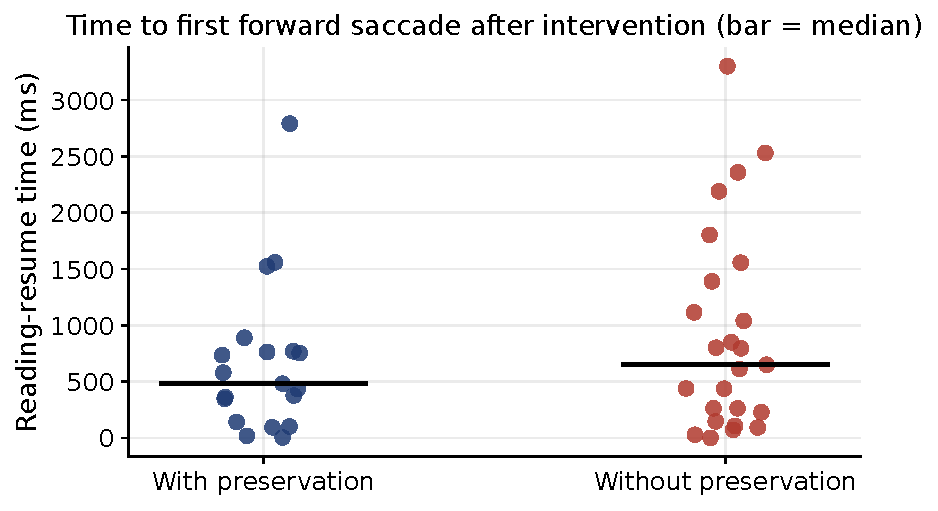
\includegraphics[width=0.48\textwidth]{figures/eval-rrt.pdf}\hfill
  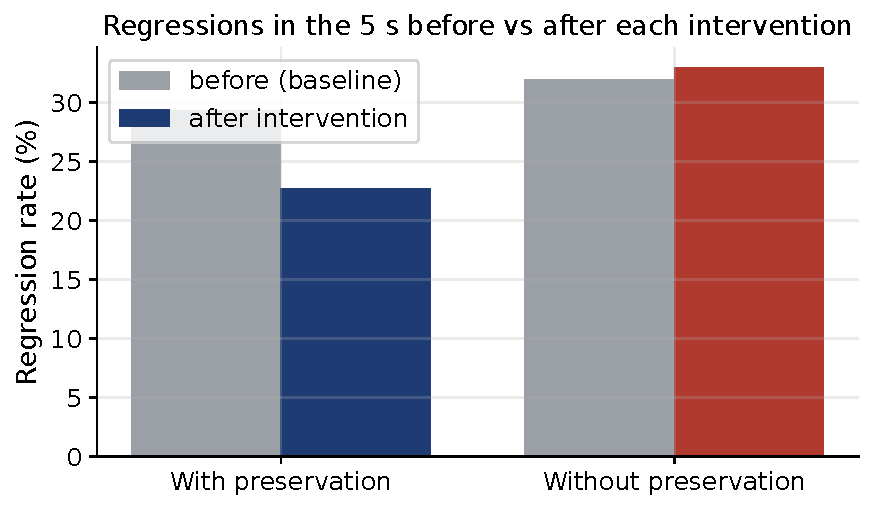
\includegraphics[width=0.48\textwidth]{figures/eval-post-regression.pdf}
  \caption{Left: reading-resume time per intervention by condition (\interventionsWith{} interventions \on{}, \interventionsWithout{} \off{}, of which one has no observation; bars mark medians); points are interventions nested within four participants, not independent observations.
  Right: regression rate in the five seconds before and after each intervention, by condition; without preservation the rate rises after the intervention, with preservation it falls below its baseline.
  Both panels are descriptive only.}
  \Description{Left, a dot plot with two columns of points, one per condition, where the with-preservation points sit lower with median bars at 482 and 650 milliseconds. Right, a paired bar chart of regression rates before and after interventions for the two conditions, showing a decrease with preservation and a slight increase without.}
  \label{fig:rrt}
\end{widefigure}

\paragraph{Record integrity.}
Auditing the exports revealed that \duplicateFixations{} of \fixationTotal{} fixation records (\duplicateFixationPct\%) and \duplicateSaccades{} of \saccadeTotal{} saccade records (\duplicateSaccadePct\%) repeat an earlier payload exactly, and a further \nearDuplicateFixations{} and \nearDuplicateSaccades{} repeat an earlier event's identity with different layout-dependent fields; gaze samples and interventions contain no duplicates.
The cause is a recording defect, since fixed: the provider resends its window of recent events every two seconds with line and token indices re-derived from the current layout, and the backend, which matched the previously newest record in full to find where the new events began, no longer recognised it after a reflow and recorded the whole window again.
Each repeat is thus the same eye movement written twice, which is why saccades, whose payload depends on two tokens, suffer more.
Discarding records that repeat an earlier event's identity gives regression rates of \regWithPreIdDedup\% before and \regWithPostIdDedup\% after an intervention \on{} against \regWithoutPreIdDedup\% and \regWithoutPostIdDedup\% \off{}, with resume-time medians unchanged, so the direction survives; exported event counts should nonetheless not be read as counts of distinct eye movements.

\paragraph{Self-measurement catches a defect.}
Within the four \on{} sessions, the reader recorded a graded outcome for every intervention: the displacement the reflow induced and the residual after the restore.
\cpDegraded{} of the \interventionsWith{} outcomes were graded degraded and \cpPreserved{} preserved, and for the degraded ones the median residual was \cpDegradedResidualMedian{}\,px against a median induced displacement of only \cpDegradedInducedMedian{}\,px.
The restore was moving readers substantially further than the reflow it compensated.
The cause was the original strategy's fixed target: it re-established the committed sentence near the top of the reading area regardless of how far the reader actually sat from it, so the smaller the reflow, the worse the compensation.

\paragraph{Browser sweep, and the revision.}
The live outcomes are observational, covering whatever interventions the participants happened to receive.
To measure displacement under controlled conditions, a harness mounts the real participant reader outside a live session (1440$\times$900 viewport, baseline typography, gaze disabled so the anchor falls back deterministically to a visible word) and drives the same restore hook over every built-in layout intervention from six page positions, recording the vertical displacement of the anchor word with preservation \off{} and \on{}.
Eleven interventions crossed with six positions give \sweepTrials{} scheduled trials; the harness was run once against the original restore and once against the revised one, and the two runs are separate browser executions rather than a matched experiment: \sweepAnchorDiff{} of the \sweepTrials{} trial keys resolved to a different anchor word across the runs, \sweepOffDiff{} differ in the \off{} displacement by more than 1\,px, and a few line-width trials lose the anchor word from the rendered page, leaving \sweepPairsOriginal{} complete pairs in the original run and \sweepPairsRevised{} in the revised run.
Table~\ref{tab:sweep} reports both runs side by side.
Without preservation the bare reflow moves the word by about one line at the median (\sweepOffMedianOriginal{} and \sweepOffMedianRevised{}\,px in the two runs; one line is 32.4\,px), with a heavy tail for large font and line-width changes.
With the original restore, preservation made displacement worse rather than better: the median rose to \sweepOnMedianOriginal{}\,px, about three times the bare reflow in the same run, the restore moved the word further than the reflow (by more than 1\,px) in \sweepOverOriginal{} of \sweepPairsOriginal{} pairs, and the effect was starkest for the smallest changes, such as a letter-spacing step that moves the word not at all being thrown 115\,px.
The revised restore returns the captured reading position to the viewport offset it held before the change (Section~\ref{sec:platform-context}); in its run it over-repositions in \sweepOverRevised{} of \sweepPairsRevised{} pairs and brings the median to \sweepOnMedianRevised{}\,px, at or below that run's \off{} baseline, with the gains concentrated where reflows are large, while line-width changes repaginate and lie beyond what a within-page restore can compensate (Figure~\ref{fig:overreposition}).
The revision is verified geometrically by this sweep; its behavioural benefit to readers has not been re-measured, and a matched benchmark with pinned anchors and rendering environment would be needed for a controlled effect estimate.

\begin{widetable}
\centering
\small
\caption{Median vertical displacement (px) of the anchor word per intervention in the browser sweep, for the run against the original restore and the run against the revised restore, each with preservation \off{} and \on{}.
Six positions per intervention; an asterisk marks cells with fewer than six measurements because the anchor word left the rendered page.
One reading line is 32.4\,px; lower is better.
The two runs resolved different anchor words in \sweepAnchorDiff{} of \sweepTrials{} trials, so compare \on{} with \off{} within a run rather than across runs.}
\label{tab:sweep}
% Generated by analysis/build_paper_assets.py; do not edit by hand.
\begin{tabular}{@{}lrrrr@{}}
\toprule
Intervention & \off{} & \on{} (original) & \off{} & \on{} (revised) \\
\midrule
Font size $+2$\,px (18 to 20) & 24.5 & 168.3 & 24.5 & 24.5 \\
Font size $+6$\,px (18 to 24) & 174.8 & 225.2 & 142.4 & 43.0 \\
Font size $-2$\,px (18 to 16) & 38.0 & 82.7 & 38.0 & 54.0 \\
Line height $+0.3$ (1.8 to 2.1) & 36.0 & 124.7 & 35.4 & 35.4 \\
Line height $-0.3$ (1.8 to 1.5) & 23.1 & 53.7 & 34.5 & 31.7 \\
Line width $-120$\,px (680 to 560) & 136.6$^{*}$ & 156.1$^{*}$ & 188.1$^{*}$ & 188.1$^{*}$ \\
Line width $+80$\,px (680 to 760) & 161.9$^{*}$ & 148.6 & 161.9$^{*}$ & 148.6 \\
Letter spacing $+0.06$\,em & 0.0 & 115.0 & 0.0 & 0.0 \\
Letter spacing $+0.12$\,em & 44.7 & 154.8 & 32.4 & 16.3 \\
Font family to Inter & 1.0 & 31.3 & 1.0 & 1.0 \\
Font family to Space Grotesk & 0.0 & 49.5 & 0.0 & 0.0 \\
\midrule
\textbf{All trials} & \textbf{32.4} & \textbf{104.4} & \textbf{34.3} & \textbf{32.4} \\
\bottomrule
\end{tabular}

\end{widetable}

\begin{figure}
  \centering
  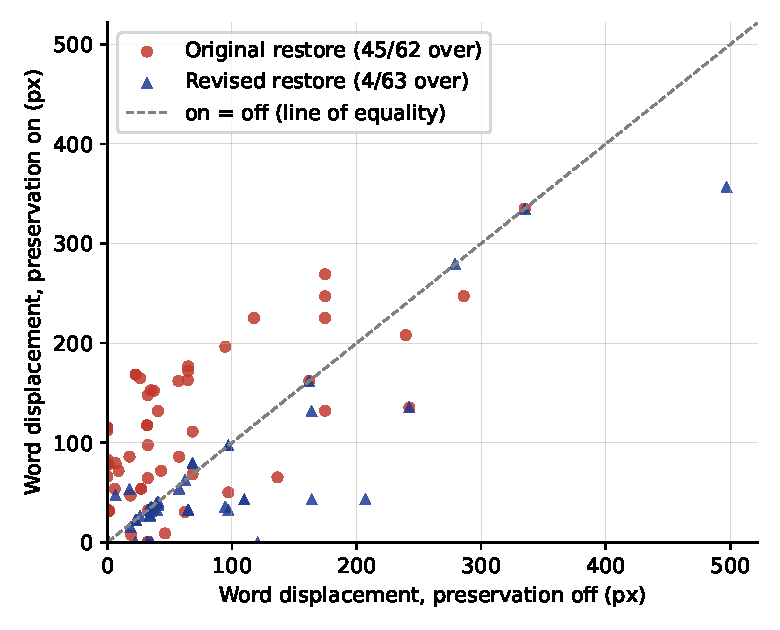
\includegraphics[width=\narrowwidth]{figures/sweep-overreposition.pdf}
  \caption{Displacement of the anchor word with preservation \on{} against its displacement \off{}, one point per complete pair (\sweepPairsOriginal{} original, \sweepPairsRevised{} revised).
  Points above the line of equality mean the restore moved the word further than the reflow alone (by more than 1\,px in \sweepOverOriginal{} pairs with the original restore, circles, and \sweepOverRevised{} with the revised one, triangles).
  The two versions were captured in separate runs.}
  \Description{A scatter plot of on-displacement versus off-displacement with a dashed diagonal line of equality. Circle markers cluster above the diagonal; triangle markers lie on or below it.}
  \label{fig:overreposition}
\end{figure}


\section{Discussion}
\label{sec:discussion}

\paragraph{What the platform enables.}
The comparisons this research area needs are now configuration rather than reimplementation: contrasting intervention presentation forms, commit boundaries, or decision strategies under identical sensing is a matter of session templates and module selection, with counterbalancing supplied by the platform's randomised item ordering and evidence supplied by the session record.
The unbundled study that our own confound calls for, crossing the revised restore with and without the highlight cue, is exactly such a configuration.
Beyond single studies, the exported records form a corpus on which an external decision provider can be trained offline and then attached through the same seam it will be judged at, closing the loop the programme's envisaged AI-driven adaptation requires \cite{dtucompute2025rtr}.

\paragraph{Measure the quality attribute you claim.}
The over-repositioning result is the strongest argument for a design principle the platform embodies: a system should measure the property it claims to provide, so it can report its failures as readily as its successes.
Context preservation was a headline feature, yet its original geometry made small reflows worse, and nothing in ordinary operation would have surfaced that; the per-intervention residual in the session record did.
The same record also surfaced the repeated derived-event payloads and the mismatch between the two sweep runs, which a success-only log would have hidden.
We suggest the principle transfers beyond reading platforms: any interface that changes state during a continuous user task can hold the change until a natural boundary, re-anchor the user's focus across it, and record what the change cost.

\paragraph{Human authority is part of the architecture.}
Manual, advisory, and autonomous modes share one proposal and intervention record, so a study can move gradually from researcher control to automation without changing the presentation runtime or losing provenance, and advisory mode lets later analysis distinguish model behaviour from operator resolution while a provider is experimental.
The current implementation is not resilient automation, however: provider detachment is recorded but does not trigger a switch to the built-in strategy, and heartbeat expiry is not enforced.

\paragraph{Limitations.}
The behavioural comparison rests on four participants drawn from the authors and acquaintances, reading two texts in an unbalanced condition order under researcher-timed manual interventions; the numbers are descriptive, and the \on{} condition bundles the restore with the highlight cue, so no causal attribution to the restore geometry is possible.
The derived event streams of the recorded sessions contain repeated records from an extraction defect that has since been traced and fixed; the regression rates are reported with and without identity-based de-duplication and keep their direction, but the sessions have not been re-recorded with the fix.
The revised restore is verified geometrically, in a sweep whose two runs are not matched, and has not been re-evaluated with readers.
The automated decision path was exercised within budget in a single advisory-mode run with a rule-based reference provider on one host, not at campaign scale or over a network, and no learned decision model has yet run against the platform.
The provider contract has one external integration, written by us around a collaborator's code; a single such integration is encouraging, not proof of independence.
Timing figures are loopback figures of the intended single-host deployment and none measures the visible endpoint.
The recorded sessions did not exercise boundary scheduling, and the exports pin the producing application version but not the full browser, font, and provider configuration, so historical provenance is incomplete.
Reading material is restricted to reflowable Markdown, and our participants were general readers, not the vision-impaired or dyslexic readers who motivate the programme, so no claim here extends to those groups.

\paragraph{Future work.}
Three studies follow directly.
First, the three-condition study separating restore geometry from highlighting on the revised mechanism, which would also replace the authors-as-participants sample and should pin texts, order, and intervention timing.
Second, a campaign-scale run of the automated decision path with a learned provider, turning the single-run check into a measured result, ideally with an end-to-end latency measurement to the display.
Third, the properly powered efficacy study the platform was built to host, asking whether specific interventions improve reading rather than only measuring their immediate cost.
On the platform side, re-recording sessions with the corrected event extraction, adding automatic fallback and heartbeat enforcement with a fault-injection test, and attracting external providers and multimodal sources behind the existing ports would push the contract from author-validated toward independently validated.

\section{Conclusion}
\label{sec:conclusion}

We asked whether the gaze-adaptive reading loop can be cleanly separated into replaceable modules under real-time conditions, and answered with a built and measured platform: a two-screen, researcher-operated system whose sensing, analysis, decision, and intervention modules sit behind contracts checked by the build, driven by a real 90\,Hz eye tracker with every client round trip of the eight sessions inside a 100\,ms budget, analysed live by a collaborator's pipeline attached through its provider contract, and recorded into replayable sessions from which every result in this paper was recomputed.
Its self-measurement exposed, and its revision geometrically removed, an over-repositioning defect in our own context-preserving restore, and the same records exposed a duplicate-recording defect in provider event extraction, since traced and fixed, and an unmatched benchmark, which is precisely the kind of finding an instrument should produce about itself.
The controlled studies this field needs next, unbundling restore geometry from highlighting, running learned decision providers at scale, and measuring efficacy for the readers who motivate the work, are configuration choices on this platform rather than rewrites of core code.


\section*{Privacy and Ethics Statement}
% CONFIRM(authors) before submission: (a) that consent was given as stated (add "written" or "verbal" if you want the form stated); (b) that no ethics-committee approval was required under DTU's rules. Both describe what the authors reported; neither has been checked against a document.
The recorded sessions were a technical evaluation of the instrument by its developers: five adult volunteers, two of them authors, were told what would be recorded and gave informed consent, no vulnerable participants or deception were involved, and the evaluation did not require approval by a research ethics committee under the rules of the authors' institution.
Gaze reveals reading ability and attention, so the platform keeps all data on the researcher's machine, transmits nothing to external services, and leaves consent, pseudonymisation, and retention as explicit obligations of the deploying researcher; the released exports carry participant codes only, with names and the eye-condition field removed.
The platform is meant to enable studies that may eventually benefit readers with vision impairment or reading difficulties, but nothing in this paper evaluates such readers, and gaze-adaptive text should not be deployed for them before studies with the affected groups have measured both benefit and cost.

\section*{Availability}
The platform, its documentation, the browser displacement harness, the anonymised session exports, and the audit script that regenerates every quantity in this paper from them are open source under the MIT licence at \anon[a public repository whose link is withheld for review]{\url{https://github.com/MrSachin7/reading-the-reader-monorepo}}.

\section*{Generative AI Disclosure}
Generative AI coding assistants (OpenAI Codex and Anthropic Claude) were used in implementing the platform, the browser harness, and the audit script, and in drafting this manuscript from the authors' thesis text; the authors reviewed and tested all generated code, revised every passage, and alone designed the architecture, the evaluation, and its interpretation.

% Real acknowledgments: acmart drops the acks environment in anonymous mode, so these appear only in the reading copy and the camera-ready.
% CONFIRM(authors): thank the supervisors here by name if they are not co-authors.
\begin{acks}
The authors would sincerely like to thank and acknowledge the Novo Nordisk Foundation for funding this research, carried out within the Reading the Reader project at DTU Compute \cite{dtucompute2025rtr, nnf2023rtr}, through a ``Data Science Collaborative Research Programme 2022'' grant with agreement No.~NNF22OC0076877.
We thank Katarina Kraljevi\'{c} and Sree Keerthi Desu for making their reading-difficulty pipeline available as the external analysis provider in the evaluation, and the volunteers who took part in the recorded sessions.
\end{acks}
% The acks environment is dropped automatically in the anonymous review build; the full
% acknowledgments appear in the reading copy and the camera-ready.

\bibliographystyle{ACM-Reference-Format}
\bibliography{bibliography}

\end{document}
